\documentclass[en]{../../../eplsummary}

\hypertitle{cloud-INGI2145}{7}{INGI}{2145}
{Houtain Nicolas}
{Canini Marco}

\section{Cloud computing}

\subsection{Introduction}

\begin{center}
\textit{Cloud computing is a model for enabling convenient, 
on-­demand network access to a shared pool of configurable 
computing resources (e.g., networks, servers, storage, 
applications, and services) that can be rapidly provisioned 
and released with minimal management effort or 
service provider interaction.}
\end{center}

\paragraph{Cloud commandments}
\begin{enumerate}
    \item Partition everything
    \item Use asynchony everywhere
    \item Automate everything
    \item Remember that everything fails
    \item Embrace inconsistency
\end{enumerate}

\paragraph{Cloud benefit}:
\begin{itemize}
    \item Elastic,  just-­in-­time  infrastructure
    \item More  efficient  resource  utilization
    \item Pay  for  what  you  use
    \item Potential  to  reduce  processing  time (parallelization)
    \item Leverage  multiple  data  centers (high availability)
\end{itemize}




\subsubsection{Hardware scalability}

Cloud need for \textbf{scalability} because modern application require
huge amounts of processing and data. Cluster (\textit{room-sized}) and datacenter 
(\textit{building-sized}) can provide the resources needed.
They are composed of \textbf{rack} which is a aggregation of storage devices, many
nodes and switch to connect nodes together. Unfortunately, they are not perfect.
\begin{enumerate}
  \item Difficult to dimension because they must be provisioning for the peak load
  \item Expensive in hardware invest, expertise (ex: special software) and maintenance
  \item Difficult to scale because adding new machines is not easy
\end{enumerate}


\subsubsection{Model}
Cloud computing is a business models where everything is a service:
\begin{itemize}
  \item SaaS: Software as a service
  \item PaaS: Platform as a service
  \item IaaS: Infrastructure as a service
\end{itemize}

\subsubsection{Types}
There also have three types of cloud : 
\begin{itemize}
  \item Public: commercial commercial service open to almost anyone.
  \item Community: shared by several similar organization
  \item Private: shared within a organization
\end{itemize}
In this course we focus on public cloud.

\subsubsection{Applications}

Typically, applications that involve large amounts of computation, storage,
bandwidth Especially when lots of resources are needed quickly or load varies
rapidly.

\begin{itemize}
  \item Web app: Near the edge of the application focus is on vast 
    numbers of clients and rapid response
  \item Processing pipelines: Inside we find data-­intensive services that 
    operate in a pipelined manner, asynchronously
  \item Batch processing: Deep inside the application we see a world of 
    virtual computer clusters that are scheduled to 
    share resources and on which applications like 
    MapReduce (Hadoop) are very popular
\end{itemize}


\subsubsection{Virtualization}
IS used to simulate multiple physical machine for the consumer with different
capabilities. It's powerful for security and isolation because VM cannot influence
other. In the other hand, performance is hard to predict because other VM run on
the same physical machine.

\subsubsection{Challenge}
\begin{tabular}{m{0.5\linewidth}m{0.5\linewidth}}
\begin{itemize}
  \item Availability
  \item Data lock-in (moving data)
  \item Data confidentiality and auditability 
  \item Data transfer bottlenecks
  \item Performance unpredictability for VM
\end{itemize}
&
\begin{itemize}
  \item Scalable storage
  \item Bugs in large distributed systems
  \item Scaling quickly
  \item Reputation fate sharing
  \item Software licensing
\end{itemize}
\end{tabular}


\section{Design for scale}

A system is scalable if it can easily adapt to 
increased (or reduced) demand.

\subsection{Parallelism programming}

\subsubsection{Vocabulary}
\begin{description}
  \item[Parallelism]: refers to techniques to make programs faster by
    performing several computations in parallel.

  \item[Concurrency]: is the composition of independently executing
    computations.
\end{description}

\subsubsection{Parallelization}
\begin{itemize}
  \item \textbf{Amdahl's law}:

    \begin{tabular}{m{0.5\linewidth}m{0.5\linewidth}}
    $$\quad S = \frac{1}{\alpha +
    \frac{1-\alpha}{N}}$$ where $\alpha$ is the sequential part and $N$ the
    number of cores.
    &
    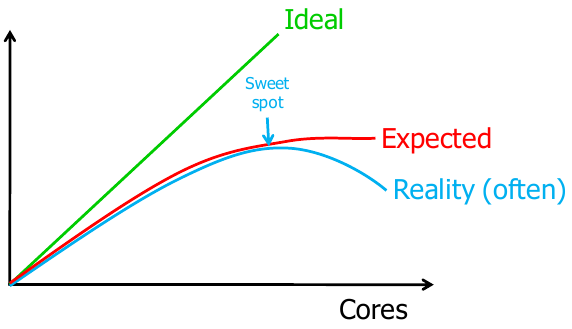
\includegraphics[width=6cm]{img/amdahl.png}
  \end{tabular}

  The coarse-grain (opposited to fine-grain) parallelism is more efficient
  because he limits the communication and coordination overheads by allow
  bigger task.
  \item \textbf{Dependencies}: Some task need to be after other which limits the degree of 
    parallelism. $\rightarrow$ Scheduling problem
\end{itemize}

\subsubsection{Synchronization and consistency}

\begin{itemize}
  \item \textbf{Sequential consistency}: the result is the same as if the
    operation are done in sequential order.

  \item \textbf{Strong consistency}: After update completes, all subsequent
    accesses will return the updated value

  \item \textbf{Weak consistency}: After update completes, accesses do not
    necessarily return the updated value;; some condition must be
    satisfied first (such as update needs to reach all the replicas)

  \item \textbf{Eventual consistency}: Specific form of weak consistency: If
    no more updates are made to an object, then eventually all reads will
    return the latest value
\end{itemize}

\subsubsection{Architecture}
\begin{itemize}
  \item Symmetric multiprocessing (SMP): all processors share same memory.
    
    \begin{tabular}{m{0.6\linewidth}m{0.4\linewidth}}
      \begin{itemize} 
        \item[+] Simplicity and easy to load balance 
        \item[-] Scalability limited and expensive
      \end{itemize}
      &
      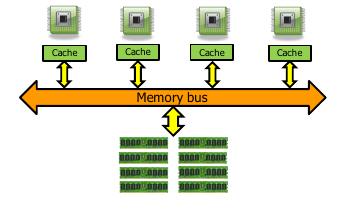
\includegraphics[width=5cm]{img/SMP}
    \end{tabular}

  \item Non Uniform memory architecture (NUMA)
    
    \begin{tabular}{m{0.6\linewidth}m{0.4\linewidth}}
      \begin{itemize} 
        \item[+] Better scalability and faster memory
        \item[-] Complicates programming and scalability limited
      \end{itemize}
      &
      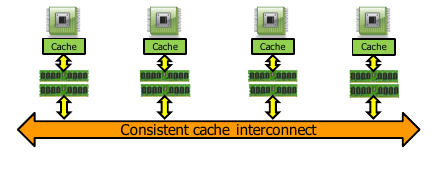
\includegraphics[width=5cm]{img/NUMA}
    \end{tabular}

  \item Shared Nothing
    
    \begin{tabular}{m{0.6\linewidth}m{0.4\linewidth}}
      \begin{itemize} 
        \item[+] Nice scalability
        \item[-] Requires different programming model
      \end{itemize}
      &
      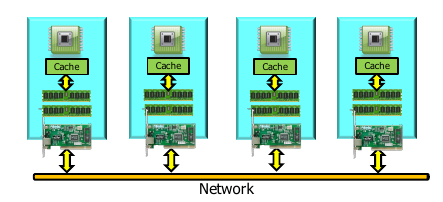
\includegraphics[width=5cm]{img/Nothing}
    \end{tabular}

\end{itemize}


\subsection{Distributed programming}

\subsubsection{Vocabulary}
\begin{description}
  \item[Faults]: Some component is not working correctly
  \item[Failure]: System as a whole is not working correctly
\end{description}

\subsubsection{Wide-area network}
The transfert speed for some data are defined by some attributs:
\begin{enumerate}
  \item Propagation delay
  \item Bottlenecks capacity on the path
  \item Queueing delay, loss, reordering, congestion, rtt 
    (take in account by TCP)
\end{enumerate}

$\rightarrow$ wide-area networks complicates the communication and faults are
more common

\subsubsection{Faults}

Fault are a common event in distributed system and some faults
are correlated.

\begin{itemize}
  \item \textbf{Crash faults}: node simply stop
  \item \textbf{Rational behavior}: owner manipulates node to increase profit
    (ex: lies on the routes to have traffic through it's own AS)
  \item \textbf{Byzantine faults}: faulty node could do anything (ex: stop, send spam,
    attack other, tell lies,...)
\end{itemize}

To prevent fault, we can \textit{prevent} them by using verification,
\textit{detect} them or \textit{mask} them by using replicas. The problem of
using \textbf{replicas} is to be able to maintain consistency between them!

\subsubsection{Consistency}

\begin{itemize}
  \item \textbf{Strong consistency}: After update completes, all subsequent
      accesses will return the updated value

  \item \textbf{Weak consistency}: After update completes, accesses do not
      necessarily return the updated value;; some condition must be satisfied
      first (such as update needs to reach all the replicas)

  \item \textbf{Eventual consistency}: Specific form of weak consistency: If no
      more updates are made to an object, then eventually all reads will return
      the latest value

  \item Causal consistency: If client A has communicated to client B that it
      has updated a data item, a subsequent access by B will return the updated
      value, and a write is guaranteed to supersede the earlier write. Client C
      that has no causal relationship to client A is subject to the normal
      eventual consistency rules

  \item Read-your-writes consistency:  Client A, after it has updated a data
      item, always accesses the updated value and will never see an older
      value.

  \item Session consistency: Like previous case but in the context of a
      session, for as long as the sessions remains alive.

  \item Monotonic read consistency: If client A has has seen a particular value
      for the object, any subsequent accesses will never return any previous
      values

  \item Monotonic write consistency: In this case the system guarantees to
      serialize the writes by the same process
\end{itemize}

We can combine them, and monotonic reads + read-your-write are most desirable
than eventual consistency.


\paragraph{Storage system example}


\begin{tabular}{m{5cm}m{12cm}}
    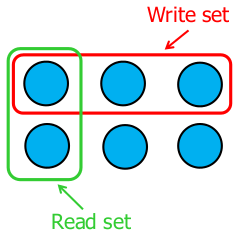
\includegraphics[width=3cm]{img/replicas} &
    
\includegraphics[width=7cm]{img/replicas2}
    \begin{itemize}
        \item[$\rightarrow$] Strong consistency
    \end{itemize} \\
\end{tabular}


\paragraph{Consensus}
\begin{enumerate}
    \item Clients send requests to each of the replicas
    \item Replicas coordinate and each return a result
    \item Client chooses one of the results, e.g., the one that is 
        returned by the largest number of replicas
    \item If a small fraction of the replicas returns the wrong result, or 
        no result at all, they are 'outvoted' by the other replicas
\end{enumerate}


\subsubsection{CAP theorem}
%TODO tikz
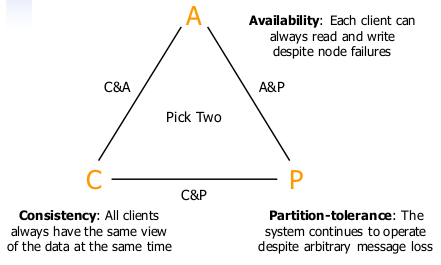
\includegraphics[width=5cm]{img/CAP}

\begin{itemize}
    \item C\&P -> Many replicas + consensus
    \item A\&P -> Many replicas + relaxed consistency
\end{itemize}

Actually, we have a lot of partition and we have a trade-off
between C and A. \textbf{ACID} (atomicity, consistency, isolation, durability)
become \textbf{BASE} (basically available, soft-state, eventually consistent).



\subsection{Structure}
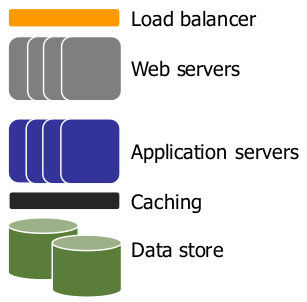
\includegraphics[width=5cm]{img/structApp}
Caching  is  central  to  responsiveness

\begin{itemize}
    \item Stateless server: Views  a  client  request  as  an  independent  
        transaction  and  responds  to  it


        Easy to scale and more robuste because instance failure does not require
        overheas restoring state

    \item Statefull server: Scaling is challenging 
        
        \paragraph{Traditionnal approach is replication}
        \begin{itemize}
            \item Data  is  written  to  a  master  server  and  then  replicated  to  one  
        or  more  slave  servers  (synchronously  or  asynchronously))
            \item Read  operations  can  be  handled  by  the  slaves
        \end{itemize}

        But in this case, master becomes the write bottleneck and single point of failure.
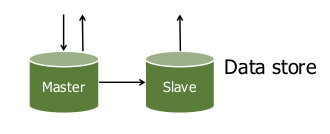
\includegraphics[width=5cm]{img/MasterSlave}

        \paragraph{Sharding with partitionning}
        Split  data  between  multiple  
        machines  and  have  a  way  to  make  sure  you  
        always  access  data  from  the  right  place. 
        Typically, define  a  sharding key  and  create  a  shard  mapping.

        Really high availability, incread read and write throughput and possibility 
        of doing more work in parallel within the application server.
        But the challenge is to find a good partitionning scheme.


        \subparagraph{} Sharging is  not  only  for  partitioning  data  
        within  a  database, but can be use to  partition  data  across  caching  
        servers (memcached, redis).
\end{itemize}

\paragraph{First-tier parallelism}
Parallelism  is  vital  for  fast  interactive  services, and 
parallel actions must focus on the critical path (it means delay that
contribute to the response delay and not asynchronous that are shortly)

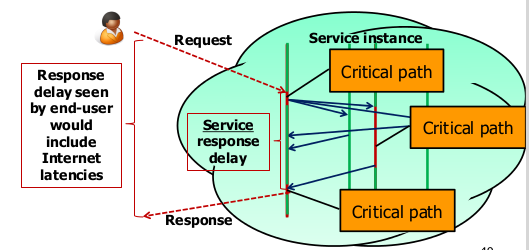
\includegraphics[width=5cm]{img/critical}


Note that update for replicas are typically done in asynchronous way, so we
might  not  experience  much  delay  on  the  critical  path.

Asynchronous  operations  decouple  systems  and  
enable  quicker  responses  at  the  expense  strong  
consistency.
Indeed, this can rise some issues which result in inconsistency:
\begin{itemize}
    \item We don't know in which order replicas applying the update
    \item The leader can crash before replicas change and lose some
        update
\end{itemize}


\section{Cloud storage}

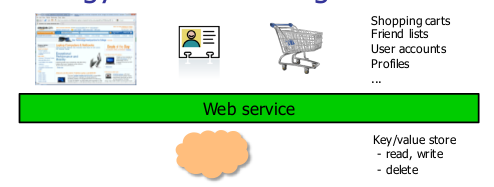
\includegraphics[width=5cm]{img/storage}
Many  cloud  services  have  a  similar  structure, 
But  the  actual  storage  service  is  very  simple (Read/write  'blocks',
similar  to  a  giant  hard  disk) and the translation  done  by  the  web  service.

\paragraph{ideal store}
\begin{itemize}
\item Perfect  durability – nothing  would  ever  disappear  in  a  crash
\item 100\%  availability – we  could  always  get  to  the  service
\item Zero  latency from  anywhere  on  earth  – no  delays!
\item Minimal  bandwidth  utilization  – we  only  send  across  the  network  what  we  absolutely  need
\item Isolation under  concurrent  updates  – make  sure  data  stays   consistent
\end{itemize}

BUT he  “cloud”  exists  over  a  physical  network (communication take time + limited bandwith)
and The  “cloud”  has  imperfect  hardware (failures)

\paragraph{Observation}
\begin{itemize}
    \item Read-­only  (or  read-­mostly)  data  is  easiest  to  support
    \item Granularity  matters:  “Few  large-­object”  tasks  generally  
        tolerate  longer  latencies  than  “many  small-­object”  tasks


        But  it’s  much  more  expensive to  replicate  or  to  update!

    \item[->] Maybe  it  makes  sense  to  develop  separate  solutions  for  large  
        read-­mostly  objects  vs.  small  read-­write  objects!
        Different  requirements  → different  technical  solutions
\end{itemize}


\subsection{Key-value stores (KVS)}


\subsection{Amazon dynamo (kind of KVS)}



\section{Paper}



\end{document}
